%!TEX root = ../dissertation.tex
\begin{savequote}[75mm]
I know words. I have the best words.
\qauthor{Donald Trump}
\end{savequote}

\chapter{Introduction}
\label{introduction}
\section{Cholinergic Systems}
\newthought{Nary a process in the mammalian body can commence without participation of cholinergic systems.} \Ac{ach} was chemically and pharmacologically described by Henry Dale more than 100 years ago\cite{Dale1914}. A short time later, Otto Loewi published the first proof of signal transmission by small molecules: he transferred physiological solutions from electrically stimulated frog hearts to naive hearts and observed their reactions; the solution that provoked a parasympathetic response he proposed to contain a »vagus substance«\cite{Loewi1921}. Finally, in 1929, Henry Dale completed the picture by isolating acetylcholine from mammalian tissue and identifying it as the molecule responsible for the parasympathetic response\cite{Dale1929}. Dale and Loewi's joint effort in »Discoveries in Chemical Transmission of Nerve Impulses« was rewarded with the »Nobel Prize in Physiology or Medicine« in 1936.

Although we have learned much about cholinergic systems in these past 100 years, our understanding of the mammalian nervous system still is fairly limited. Even when disregarding peripheral nervous systems, the complexity of cholinergic transmission is immense, and a myriad functions have been attributed to cholinergic circuits in the \ac{cns}. Central nervous projections of cholinergic fibres were extensively mapped by M. Marsel Mesulam and others in the 1980s\cite{Mesulam1984}, with a majority of long projection neurons originating in one of the eight cholinergic nuclei, Ch1-Ch8. While many of these anatomical structures have been filled with meaning by associations with both rudimentary as well as higher brain functions, there are still as many cholinergic pathways whose function is entirely unclear (Figure \ref{fig:projections}, from my first manuscript\cite{Lobentanzer2019a}).

This holds particularly true for the only recently discovered cortical cholinergic interneurons, which, in comparison to their projecting counterparts, are very small and numerically vastly inferior to other neuron types in the cortex. Thus, their detection and analysis with current methods is challenging. 

\begin{figure}
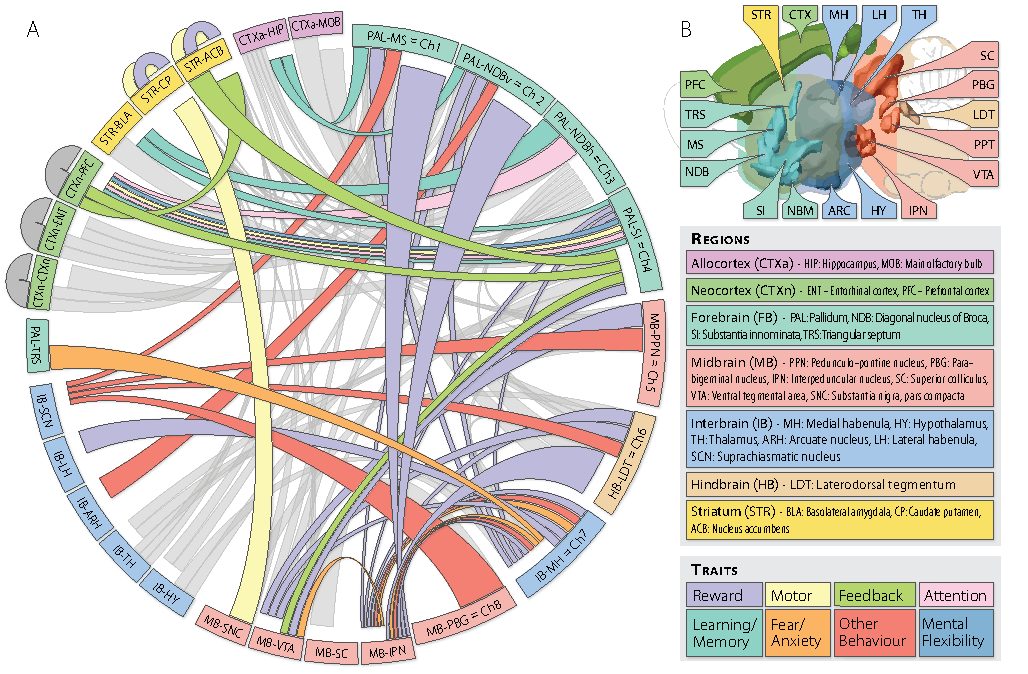
\includegraphics[width=\textwidth]{figures/projections}
\caption[Short figure name.]{This is a figure that floats inline and here is its caption.
\label{fig:projections}}
\end{figure}

\subsection{Cholinergic Aspects of Disease}
\newthought{Cholinergic systems are integral for a myriad physiological functions}, and as such they are critically involved in aetiologies and phenotypes of a number of central and peripheral diseases. Of interest to this dissertation are the cholinergic aspects of degenerative and non-degenerative central nervous diseases (such as Alzheimer's Disease, Bipolar Disorder, Schizophrenia), ischemic conditions in stroke, and peripheral modulation of immune responses, particularly in the context of the aforementioned diseases.

\subsubsection{Alzheimer's Disease}
Cholinergic progression

Monotherapeutic approaches

\subsubsection{Schizophrenia and Bipolar Disorder}
Dirty therapeutics, multitarget

\subsubsection{Stroke}

\subsubsection{Immunity}

\subsection{Neurokines} \label{sec:intro:neurokine}
In comparison to the widely studied cholinergic projection neurons originating in the basal forebrain (Ch1-Ch4) that are known to depend on a retrograde survival signal by means of \ac{ngf}, trophic influences on other cholinergic populations such as the cortical interneurons are unclear.  \ac{ngf} was described by Rita Levi-Montalcini in the 1950s as the first known instance of trophic peptides required for the survival of sympathetic ganglia\cite{Levi-Montalcini1960}, and the dependence of basal forebrain cholinergic neurons on retrograde \ac{ngf} signalling was discovered in the 1980s\cite{Hefti1986}.

A second group of trophic peptides with cholinergic implications are the so-called »neurokines«; the name results from the fact that this particular subgroup of cytokines has been associated with neuronal function in the central and peripheral nervous systems. Most prominently they include the \ac{cntf}, \ac{lif}, and \ac{il}, all of which coincidentally have been known under the acronym CDF. In the end of the 1980s, two groups of scientists (McManaman\cite{McManaman1988} and Rao\cite{Rao1992}) independently identified proteins in extracts of muscle fibre that induced a differentiation of neurons towards a cholinergic type, and thus termed these proteins »choline acetyltransferase development factor« or »cholinergic differentiation factor« (both abbreviated CDF). Only later, through sequencing of the peptides, it became known that they had in fact discovered two distinct neurokines, \ac{lif} (Rao) and \ac{cntf} (McManaman, personal communication). \ac{il}, on the other hand, is abbreviated CDF for an entirely different reason: in this case it is short for »CTL (cytolytic T lymphocyte) differentiation factor«.

\ac{cntf}, \ac{lif}, and \ac{il} convey their impact on neuronal activity through a partly redundant neurokine receptor pathway\cite{Berger2014}. There are two basic types of neurokine receptors: soluble and transmembrane. The primary receptors for \ac{cntf} (\acs{cntfr}) and \ac{il} (\acs{ilr}) are soluble proteins that are secreted into the extracellular space and, upon binding of a neurokine, bind to transmembrane receptor dimers on the cell surface. These transmembrane receptors are the LIF receptor (\acs{lifr}) and the »interleukin 6 signal transducer« (\acs{ilst}, also known as \acs{gp}). Every neurokine has its preferred constellation of soluble and transmembrane receptors: \ac{cntf} binds to the soluble \ac{cntf} receptor and a dimer consisting of one \ac{gp} and one \ac{lifr} protein; \ac{il} binds to the soluble IL6R and a dimer of two units of \ac{gp}; \ac{lif} does not usually bind a soluble receptor but rather binds immediately to a dimer comprising one of each \ac{gp} and \ac{lifr}; however, there is significant redundancy and crosstalk between those systems\cite{Rawlings2004,Nathanson2012}.

All receptor constellations result in a main effect of activation of the \acs{jak}/\acs{stat} cascade (Fig. \ref{fig:neurokine}). More specifically, neurokines can activate \acfp{jak} 1 and 2 or the homologous \ac{tyk} 2, and, successively, \ac{stat} (»signal transducer and activator of transcription«) isoforms 1, 3, 5A, and 5B, which then convey a multitude of cellular effects (e.g. in immunity or differentiation) through transcriptional activation. The \ac{stat} cascade is inherently self-limiting in that it usually leads to expression of transcription factors that serve as repressors of the \ac{stat} genes (XXX)\cite{}. 

Neurokines, particularly \ac{il}(?), might serve as a link between the immunological and cholinergic aspects of physiological or disease processes.\todo{elaborate}

\begin{figure}
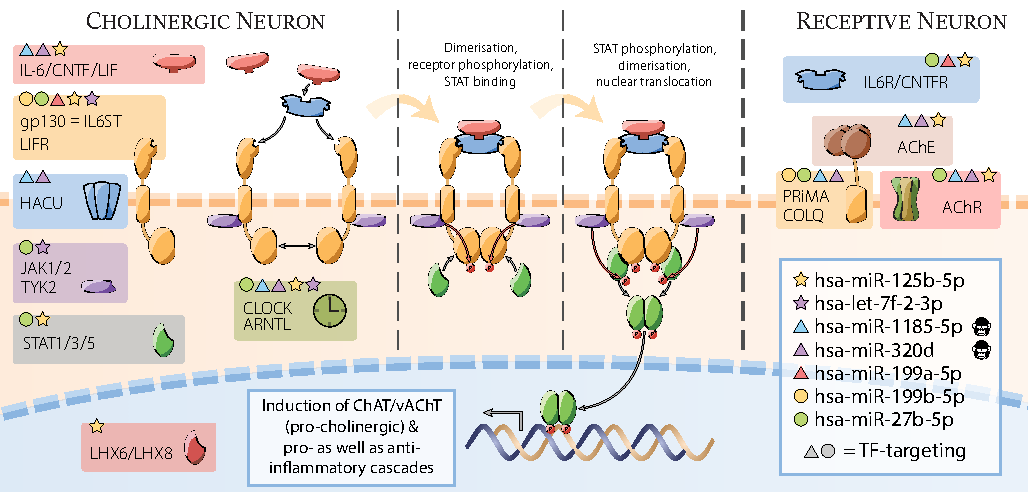
\includegraphics[width=\textwidth]{figures/neurokine}
\caption[Short figure name.]{This is a figure that floats inline and here is its caption.
\label{fig:neurokine}}
\end{figure}

%Neuronal activity is profoundly modified by cytokines

%Li Gan - NFkB activation by tau
% - Ikkbeta knockout corrects STAT1 DE

%Oleg Butovsky - TGFbeta as master glia regulator

\section{Transcriptional Connectomics}
The term »connectomics« is not strictly limited to one scientific discipline; it is frequently used when the studied matter is defined by complex relationships between interaction partners. The most frequent use outside of transcriptional matters is neuronal connectomics, i.e., the relationships and projections between brain regions. In this dissertation, connectomics generally refers to epi\-/transcriptional interaction, the processes surrounding protein-coding gene expression. For the sake of simplicity, in this dissertation all descriptions of genomics and transcriptomics matters, of genes and their small RNA regulators, are to be seen in the context of \textit{Homo sapiens}, unless explicitly stated otherwise.

\newthought{No matter their location, cholinergic neurons are defined by their ability to synthesise \ac{ach} and release it to neighbouring cells to a certain effect.} To fulfil this task, two particular proteins are essential: the \ac{chat} to synthesise \ac{ach} from choline and acetyl-Coenzyme A, and the vesicular acetycholine transporter (\acs{vacht}, official gene symbol \acs{slc}), which concentrates \ac{ach} in vesicles for later release. A notable genetic feature connects these two proteins beyond their functional association: the small \textit{\ac{slc}} gene (2420 nucleobases) sits inside the first intron of the \textit{\ac{chat}} gene and thus is already included in its primary transcript, and is subject to the \textit{\ac{chat}} promoter. However, oftentimes the (mature) transcript levels of \textit{\ac{chat}} and \textit{\ac{slc}} mRNA seem to be independently regulated; from the perspective of the organism, the possibility of differential regulation between these two genes makes sense. Since \textit{\ac{slc}} does not possess its own promoter, this differential regulation has to be conveyed epigenetically. 

This dissertation deals in large parts with approaches aiming to decipher these interactions; and while its primary topic revolves around cholinergic systems, the methods described in the following are designed to be applicable to the entirety of the genome/epigenome. Four particular types of cellular actors are subjects of these methods and therefore will be briefly introduced: genes in the classical sense as the conveyors of cellular function by encoding for proteins; \acp{tf}, a subclass of protein coding genes that are able to regulate the expression of other genes; \acp{mir}, a class of \ac{smrna} that has been known for approximately two decades and is reasonably well described functionally and mechanistically; and \acp{trf}, a second class of regulatory \ac{smrna} that has only recently been rediscovered and is significantly less well described regarding its functionality.

\subsection{Transcription Factors} \label{sec:intro:tf}
\Acfp{tf} were among the first intracellular regulatory mechanisms to be discovered (the earliest article referencing the term »transcription factor« in its title on PubMed was published in 1972). \acp{tf} commonly translocate from the cytosol into the nucleus upon activation (often by phosphorylation), where they bind specific DNA sequences that usually range in size from 6 to 12 nucleobases. The regions containing these binding sites (about 100 - 1000 bases in size) determine the effect upon binding, which can be one of two main modes: either a promoter, leading to an increased activity of transcription in the downstream vicinity of the binding site, or a repressor, having the opposite effect. 

There exists a vast body of knowledge on \ac{tf}-interactions with genes, mostly due to the long period of time since their discovery and the multitude of scientific publications, most often studying single \acp{tf} and their interactions with few genes, but cumulatively curated by several organisations. One of the currently largest curations of \ac{tf} data, TRANSFAC, saw its original release in 1988. While these curation efforts can be extensive, they may present with serious bias towards particular \acp{tf} that might hold more scientific interest and thus are published far more frequently than others. Recently, comprehensive efforts have extended the available data significantly. Driven by the advent of \ac{seq}, computational approaches have become able to not only comprehensively predict \ac{tf}-gene interactions, but to do so in a highly tissue-specific manner (see Section \ref{sec:database:tf}). The human body is estimated to express up to 2600 distinct DNA-binding proteins, most of them presumed \acp{tf}\cite{Babu2004}, although other studies give lower estimates. 

\subsection{microRNAs} \label{sec:intro:mirna}
\newthought{The first endogenous »small RNA with antisense complementarity«} was described in 1993\cite{Lee1993}, but \acfp{mir} were only recognised as a distinct regulatory class of molecules in the early 2000s. They are typically between 18 and 22 nucleobase-long, single stranded RNA fragments, and their function is now largely undisputed: \acp{mir} serve as targeting molecules for a protein complex whose primary purpose is to repress translation of mRNA, and, in some cases, lead to mRNA degradation. The complex, therefore, is called \ac{risc}; central to its function is the family of \ac{ago} proteins, which can bind the mature \ac{mir} and orient it for interaction with its targets. Guidance of \ac{risc} to the target mRNA is generally mediated via sequence complementarity between \ac{mir} and the targeted mRNA. Specifically, a »seed« region, usually bases 2-8 on the \ac{mir}, is mainly responsible for the interaction; in case of perfect complementarity of this seed to the mRNA sequence, the interaction is considered »canonical«.

In early \ac{mir} research, the 3' \ac{utr} of the mRNA was believed to contain most \ac{mir} binding sites due to its greater accessibility (i.e., the lack of active ribosomes); however, cumulative recent reports suggest that binding inside the coding region of the mRNA is a regular occurrence(cite). The rules governing \ac{mir} binding to target sequences show considerable flexibility; a recent study shows about 30\% of analysed relationships to be of »non-canonical« nature(cite). In those cases, seed pairing with the mRNA is often imperfect. To ameliorate this loss of stability, compensation occurs typically by a secondary complementary structure after a small gap of non-complementary bases, leading to a »bridge«-type constellation. \todo{FIGURE?} This flexibility has implications in applications involving targeting algorithms; those that consider only the seed region are more prone to false negatives than models that consider, for instance, the free energy of the whole molecule (see Section \ref{sec:database:mirna}).

\subsubsection{Biogenesis}
\acp{mir}, similar to coding genes, are transcribed from loci on the genome, many inside introns or even exons of coding genes\cite{Rodriguez2004}. The primary transcript (primary \ac{mir} or pri-\ac{mir}) typically contains a hairpin-like structure that usually results in a double-stranded molecule because of internal complementarity, and can contain up to six mature \acp{mir}. This hairpin structure is recognised by the DGCR8 protein (DiGeorge Syndrome Critical Region 8, in invertebrates called »Pasha«); the complex then associates with the RNA-cleaving protein »Drosha«, which removes bases on the opposite side of the hairpin, creating a \ac{mir} precursor (or pre-\ac{mir}), which is subsequently exported from the nucleus by the shuttle protein Exportin-5. In a final step in the cytosol, the ribonuclease »Dicer« removes the loop joining the 3' and 5' arms of the pre-\ac{mir}, resulting in a duplex of mature \ac{mir}, about 20 nucleotides long. Initially, it was thought to contain only one active \ac{mir}, resulting in a designation of »\ac{mir}*« for the complementary strand (commonly, the strand with lower expression). However, this notion has been disproven, and to reflect the possibility of both strands performing \ac{mir} functions, nomenclature has changed to specify the arm of the pre-\ac{mir} from which the mature form originates (suffix »-3p« for the 3' arm, and »-5p« for the 5' arm).

\ac{mir} genes, in the same way as protein coding genes, can be subject to promoters and repressors, adding another layer of expression control by \acp{tf}. However, these \ac{tf}-\ac{mir} relationships are far less well described than common coding gene interactions, because \acp{mir} due to their shortness are not amenable to many standard gene expression assay forms. Estimation of the number of distinct gene targets of any one \ac{mir} varies widely; however, it is generally accepted to not be less than several dozen targets per \ac{mir}, and up to thousands of genes per \ac{mir} (although that estimate might be overenthusiastic).

\subsubsection{Organisation and Curation}
\acp{mir} are organised and curated by means of a periodically updated web-based platform, miRBase\cite{Kozomara2019}. For \textit{Homo sapiens}, miRBase v21 contains 2588 mature \acp{mir} from 1881 precursors. Evolutionarily, the \ac{mir} repertoire has grown from rodents to primates, resulting in a number of primate-specific \acp{mir} that may convey additional function. \ac{mir} nomenclature is organised\cite{Ambros2003} in a way that assigns evolutionarily conserved \acp{mir} the same designation (number) in all species in which they are expressed. In their full names, a prefix stating the organism of origin is added; for example, hsa-miR-125b-5p (for \textit{Homo sapiens}) and mmu-miR-125b-5p (for \textit{Mus musculus}) share the same sequence and most of their functionalities.

\acp{mir} are subcategorised in families (designated »mir« with lowercase »r«) by their genomic origin and phylogenetic homology aspects. As the annotation itself, family affiliations are in flux and change with each miRBase version. miRBase v21 lists 151 distinct \ac{mir} families with 721 individual members in total. The remaining 1867 \acp{mir} do not (yet) belong to a larger family; the majority (80\%) of those is newly discovered, as indicated by a 4-digit designation number.

\subsubsection{Disease Association}
\acp{mir} have been associated with a number of \ac{cns} diseases, including \ac{ad}, \ac{pd}, \ac{bd}, and \ac{scz}. However, the largest contribution since their discovery by far has been made by cancer research; of the approximately \num{90000} publications found on PubMed with the term \ac{mir}, about \num{42000} involve cancer (search term »\ac{mir} AND cancer«). In comparison, »\ac{mir} AND Alzheimer's Disease« results in about 600 hits, while a search for »\ac{mir} AND Schizophrenia« yields just 363 publications (as of October 2019).

In \ac{ad}, several groups of \acp{mir} have been found to show characteristic perturbations before the onset of symptoms, which makes them interesting biomarker candidates\cite{Salta2017a}. Some \acp{mir} have been extensively studied in a variety of contexts, most prominently hsa-miR-132-3p. Among its targets are several key neuronal regulators (e.g. FOXP2, FOXO3, P300, MeCP2), and it is in turn controlled by many pivotal neuronal elements (e.g. REST, ERK1/2, CREB)\todo{add to abbreviations?}; this presents an explanation for the many physiological and pathological situations that miR-132-3p has been found to play a role in. Its functions include the control of neuronal survival/apoptosis, migration and neurite extension, neuronal differentiation, and synaptic plasticity. 

\acp{mir} are able to fulfil their regulatory purpose in a context- and cell-type-dependent manner\cite{Lu2015}, such that the perturbation of one single \ac{mir} might provide different functional outcomes in different tissues (e.g., glial cells and neurons), or different stages of disease. However, this »jack-of-all-trades« behaviour also poses significant problems in establishing \acp{mir} as pharmacological targets: In the case of antagonising of mimicking an existing \ac{mir}, the amount of off-target effects would not only be enormous, the entire definition of an off-target effect would continuously change between tissues and during the course of the disease. For this reason, the design of custom oligonucleotides with limited capabilities might be preferable in the development of therapeutics based on RNA interference (See also Section \ref{sec:discussion:therapy}).

\todo{Prediction?}

\subsection{Transfer RNA Fragments}
\newthought{\Ac{trna} breakdown products have been known for decades}, with first descriptions in the 1970s; back then, they were associated with a higher turnover of \ac{trna} in cancer cells\cite{Borek1977}, and proposed as urine-based biomarkers for certain malignancies\cite{Speer1979}. However, their genesis was attributed to random processes, and due to lacking molecular biology characterisation techniques, interest in those fragments quickly faded. It was not until recently that studies have shown \ac{trna} to be a major source of stable expression of small noncoding RNA\cite{Cole2009,Lee2009} in most mammalian tissues. Indeed, replicating the reports from the 1970s, \ac{trna} breakdown products are the dominant form of small RNA in secreted fluids, such as urine and bile, and make up large parts of other bodily fluids as well\cite{Godoy2018}. They exist in two major forms: \acp{tirna}, and the smaller \acfp{trf}. \textit{from stroke paper} \acp{tirna} derive from either end of the \ac{trna}, and are created by angiogenin cleavage at the anticodon loop\cite{Yamasaki2009,Ivanov2011}. Smaller fragments are derived from the 3’ and 5’ ends of the \ac{trna} (3'-\ac{trf}/5'-\ac{trf}) or internal \ac{trna} parts (i-\ac{trf}), respectively, and may incorporate into \ac{ago} protein complexes and act like \acp{mir} to suppress their targets\cite{Burroughs2011,Kumar2014}.

However, there is considerable controversy about the generalisation of \ac{trf} functions, as distinct publications discover very different and sometimes opposing mechanisms of action for their respective fragments. An obvious assumption is the \ac{mir}-like functionality, at least for those \acp{trf} that are in the length range of \acp{mir}. There have been several instances of \acp{trf} proven to act as \ac{mir}-like suppressors of translation in a \ac{risc}-associated manner\cite{Kumar2014}, and of Dicer playing a large part in their biogenesis\cite{Cole2009}. There are even instances of small RNA molecules previously mislabeled \acp{mir} that have been discovered to actually be \ac{trna}-derived, such as miR-1280\cite{Huang2017}.

On the other hand, multiple groups have identified \acp{trf} to function not in an antisense\-/complementary manner, but by homology aspects. A valine-derived \ac{trf} was found to regulate translation by competing with mRNA directly at the binding site at the initiation complex and thereby displacing the original mRNA, leading to its translational repression\cite{Gebetsberger2017}. Others have found multiple classes of \acp{trf} derived from glutamine, aspartate, glycine, and tyrosine \acp{trna}, that displace multiple oncogenic transcripts from an RNA-binding protein (YBX1), conveying tumor-suppressive activity\cite{Goodarzi2015}. Most counterintuitive is the recent finding of a \ac{trf} proven to bind to several ribosomal protein mRNAs and enhancing their translation, and, when specifically inhibited, leading to apoptosis in rapidly dividing cells\cite{Kim2017}.

There is no consistent nomenclature yet to describe and organise \acp{trf}, which are by nature more heterogeneous than \acp{mir}; while only 61 mature \acp{trna} are required in a cell to achieve a one\-/to\-/one »codon$\to$amino acid« translation, one \ac{trna} molecule can be the origin of several hundred distinct \ac{trf} molecules. Additionally, the amount of human \ac{trna} genes is estimated at 500-600\cite{Parisien2013}, and there are many more pseudo-\ac{trna} genes. To communicate the identity of individual \acp{trf}, multiple approaches are common in current literature; most prominently, \acp{trf} are tied to the parent \ac{trna} and the amino acid carried by this \ac{trna}. To illustrate: The 22-nucleotide-long LeuCAG3′ \ac{trf} (meaning: a fragment of 22 bases starting at the 3' end of the leucine-carrying \ac{trna} with anticodon »CAG«) was shown to play an important role in regulating ribosome biogenesis\cite{Kim2017}. Since there is no repository of the likes of miRBase yet, this approach can be cumbersome for replication purposes, and explicit statement of the exact sequence of each fragment is a must in publication. In fact, since the aforementioned paper does not mention the sequence explicitly, there exist 6 distinct possibilities of fragments fitting this description. While manageable on this small scale, this system prohibits efficient analysis of larger sets of \acp{trf} that cannot be individually controlled. For this reason, the approach of Loher and colleagues\cite{Loher2017} might be preferable: they propose the generation of a "license plate" based on the sequence of the fragment directly, composed of the prefix »\ac{trf}«, the length of the fragment, and a custom oligonucleotide string encoding (e.g., »B3« stands for »AAAGT«). This way, \ac{trf} names are unique and unmistakably linked to the sequence, nomenclature is species-independent, and \ac{trna} origin can be quickly determined by sequence lookup.

\todo{Disease?}

? Levels of \acp{trf} may be modulated even more rapidly than levels of \acp{mir}, since \ac{trna} molecules are very abundant in the cell and generation of mature \acp{trf} requires only enzymatic degradation of \ac{trna} but no de-novo transcription of the molecule in the nucleus (citation).

\section[Nested Multimodal Transcriptional Interactions - The Need for Connectomics]{\nopagebreak{Nested Multimodal Transcriptional Interactions\\ \qquad \qquad - The Need for Connectomics}}
The ultimate aim of transcriptional connectomics is the combination of all interacting cellular components in a model that satisfactorily explains our real-life observations and is able to predict the functional outcome of a modification of one of these players. Even in the simplified case of only studying the interactions between coding genes, \acp{tf}, \acp{mir}, and \acp{trf}, the complexity of the required model exceeds our current capabilities by far. The more we know about the functioning of these intertwined systems, the more we understand how much there is still to learn. 

For example, only recently has it become clear how complex transcriptional regulation by means of \acp{tf} really is, and, incidentally, the two systems studied foremost in this dissertation (nerve and immune cells) are the two most transcriptionally complex systems in any mammal. Through study of comprehensive genomic information of 394 tissue types in approximately 1000 human primary cell, tissue, and culture samples (from the FANTOM5 consortium) it was estimated that the mean number of active \acp{tf} towards any given gene is highest in immune (12 \acp{tf} per gene) and nervous cells (10 \acp{tf} per gene), and that any one \ac{tf} in nervous and immune cells controls expression of a mean of 175 and 160 genes, respectively\cite{Marbach2016} (see also Section \ref{sec:database:tf}). 

Similarly, it has been found that \acp{mir}, particularly in the nervous system, possess a much higher tissue specificity than coding genes, resulting in an expression landscape that varies widely between individual neuron types that are in close proximity in the brain. With the exception of single cell \ac{seq}, no modern analysis method is capable of a resolution appropriate for accurate characterisation of these expression patterns, resulting in extinction of the signal of \acp{mir} that are not expressed consistently across cell types (similar to »housekeeping« genes) because of statistical interference. Very recent studies show that \ac{mir}-gene co-expression networks are tightly linked to cell types in the nervous system, and that groups of miRs as functional modules associate with particular phenotypes in developmental and mature states\cite{Nowakowski2018}. This functional association with cell phenotype was found in quality comparable to the expression patterns of \acp{tf}, yet in quantity conveys smaller impact and thus is thought to be a fine-tuning mechanism, subtle and precise in purpose. 

Another aspect of the tissue specificity of \ac{cns}-associated \acp{mir} is the high likelihood of under-representation or even non-discovery of those very specifically expressed \acp{mir}. Adding to the problem is the experimental bias towards rodent models when it comes to thorough studies of the \ac{cns}, where human or other primate samples are a rarity compared to rats or mice. Assessments of the numbers of yet unknown novel primate- and tissue specific \acp{mir} estimate their magnitude in the thousands\cite{Londin2015}, resulting in an effective doubling of currently known \acp{mir}.

These high numbers of potentially interacting players present computational challenges: If estimating the number of expressed genes in a human cell at \num{20000} (and the number of \acp{tf} at a low 1000), this makes for an estimated minimum of \num{200000} »real« interactions in the possible $ C = \frac{1000!}{10!(1000-10)!} \cdot \num{20000} $, which practically equals infinity; this is without accounting for different tissue types or cell states (e.g., differentiation or disease). Similarly, the amount of mature \acp{mir} (2588 in miRBase v21) and their ability to target even more distinct transcripts than \acp{tf} with one single molecule present immense computational requirements for even listing all possible or actual relationships. An interaction table describing targeting of genes by \acp{mir} in one type of tissue has $ 2588 \cdot \num{20000} \approx \num{50000000} $ individual fields.

Combining the different modes of transcriptional interaction presents additional challenges. A simple model system to visualise (in only one type of cell) the interaction of \acp{tf} targeting genes, and of \acp{mir} targeting genes as well as \acp{tf}, contains about \num{20000} genes (a subset of which of the size of about 2000 are \acp{tf}), 2588 mature \acp{mir}, and a total of $ 2588 \cdot \num{20000} + 2000 \cdot \num{20000} \approx \num{90000000} $ potential interactions. In standard application scenarios, such as the generation of an interaction network around a group of genes (e.g., the cholinergic genes), the processing requirements grow linearly with each added interaction partner, and exponentially with every regulatory layer that is added. \todo{example of standard interaction gene x miR x TF}

Practically, this information has to be provided, gathered, and integrated, which further multiplies the amount of storage and processing power required. miRWalk 2.0, a collection of \ac{mir} interaction data, has collected 12 of the most popular \ac{mir}-targeting prediction datasets, each of which has their strengths and weaknesses (see \ref{sec:database:mirna}). Experimentally validated interactions (e.g. as collected in DIANA TarBase or miRTarBase) are gold standard, but far from comprehensive and strictly speaking only relevant for the cellular context in which the experiment was originally performed; there are also different evidence qualities to be accounted for, depending on the type of experiment performed. Ideally, all of these data are still accessible when performing the analysis, so a database created for this purpose should be able to incorporate all this information without any data loss while still remaining feasible in terms of computation time as well as space and working memory requirements. 

This dissertation will first describe the creation of such a database and what has been learned during its various stages, and then go on to apply the database to different biological problems from real world experiments, such as the cholinergic differentiation of human male and female cultured neuronal cells, and the blood of stroke victims.